\chapter{Conclusion}			\label{Sec:Conclusion}


In this chapter we conclude our work on the PLGD model (\ref{Eqn:PhaseLift-P-GD}) and the \emep.
Section \ref{Subsec:Conclusion-performance_results} demonstrates the effectiveness of the IRAM with adaptive parameter selection (Algorithm \ref{Alg:adaptive_IRAM}) for a variety of noisy phase retrieval problems.
Section \ref{Subsec:Conclusion-contrib_and_future} summarizes the contributions made in this dissertation and suggests possible future work.



\section{Performance results} 			\label{Subsec:Conclusion-performance_results}


This section demonstrates the efficiency of the IRAM with adaptive parameter selection (Algorithm \ref{Alg:adaptive_IRAM}) for solving the \emep.
We begin by demonstrating that Algorithm \ref{Alg:adaptive_IRAM} is more efficient than the original IRAM (Algorithm \ref{Alg:IRAM}) parameter settings for a variety of PLGD models with Gaussian noise (\ref{Eqn:PhaseLift-GD_Gaussian_noise}).
We observe that Algorithm \ref{Alg:adaptive_IRAM} typically reduces the number of matrix-vector products in the EMEP by at least $50\%$ as compared with the original IRAM settings.
Next, we show that Algorithm \ref{Alg:adaptive_IRAM} is nearly optimal as a method for choosing the ideal number of requested eigenvalues $r_k$ corresponding to the minimum number of matrix-vector products necessary for each EMEP iteration.
Finally, we demonstrate that the Arnoldi decomposition (\ref{Eqn:Arnoldi_decomp}) size parameter $m = 40$ for Algorithm \ref{Alg:adaptive_IRAM} strikes a proper balance between increasing computational efficiency and minimizing data storage.
Note that all experiments in this section are performed using termination conditions (\ref{Eqn:term_crit_new-primal_difference}) and (\ref{Eqn:term_crit_new-dual_difference}) established in Chapter \ref{Sec:PLGD_term_crit}.
All experiments are available for reproduction.\footnote{\url{https://github.com/Will-Wright/low-rank-opt-rapid-eig}}


%\subsection{Performance results for two EMEP methods}  			\label{Subsubsec:Conclusion-gen_perf_results}


We begin by comparing the performance of Algorithm \ref{Alg:adaptive_IRAM} and the original IRAM parameter choices for a variety of randomly generated and image-based phase retrieval problems.
Figure \ref{Fig:Numerics-ada_vs_orig_various_params} depicts a set of experiments with randomly generated signals.


\begin{figure}[H]
\centering
\hbox{\hspace{-1.8cm} 
	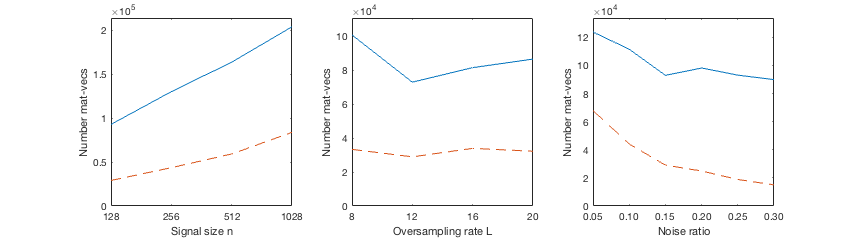
\includegraphics[scale=0.6]{Numerics-ada_vs_orig_various_params}
			}
	\vspace{0.0cm}
	\caption{
	Performance results for PLGD models with Gaussian noise (\ref{Eqn:PhaseLift-GD_Gaussian_noise}), where signals are complex with standard Gaussian distribution (\ref{Def:Gaussian_distribution_complex}).
	Results indicate Algorithm \ref{Alg:adaptive_IRAM} (dashed line) and the original IRAM parameters $m=20$, $r = 2$ (solid line). 
	Each result is the mean of 10 experiments.
	Left: Varying signal size $n$, with fixed noise ratio $\epsilon_\text{rel} = 0.15$ and oversampling scaled logarithmically with $n$ (i.e., $L = 10, 12, 12, 14$) as indicated in Theorem \ref{Thm:PhaseLift_approx}.
	Middle: Varying oversampling rate $L$, with fixed signal size $n = 128$ and noise ratio $\epsilon_\text{rel} = 0.15$.
	Right: Varying noise ratio $\epsilon_\text{rel}$, with fixed signal size $n = 128$ and oversampling rate $L = 10$.
	}
\label{Fig:Numerics-ada_vs_orig_various_params}
\end{figure}
% experiments.figure.noisyimage_comparison_adaptive_vs_orig

Figure \ref{Fig:Numerics-ada_vs_orig_various_params} demonstrates that Algorithm \ref{Alg:adaptive_IRAM} requires fewer matrix-vector products than the original IRAM parameters for the \emep \ for a wide range of phase retrieval problems.
The left and middle plots in Figure \ref{Fig:Numerics-ada_vs_orig_various_params} suggest that Algorithm \ref{Alg:adaptive_IRAM} requires about $60\%$ fewer matrix-vector products regardless of signal size $n$ or oversampling rate $L$.
Additionally, the right plot in Figure \ref{Fig:Numerics-ada_vs_orig_various_params} suggests Algorithm \ref{Alg:adaptive_IRAM} may reduce matrix-vector products by $80\%$ or more for problems with significant noise.


We also find that Algorithm \ref{Alg:adaptive_IRAM} is more efficient than the original IRAM settings for image-based phase retrieval problems.
Table \ref{Tab:Numerics-ada_vs_orig_large_images} shows the performance results for two larger images from Figure \ref{Fig:Numerics-large_images}.



\begin{table}[H]
\centering
\begin{tabular}{ |ccc|c|cc|cc| }
 \hline
			&&&  Original
			&  \multicolumn{2}{c|}{Algorithm \ref{Alg:adaptive_IRAM}}
			&	\multicolumn{2}{c|}{Algorithm \ref{Alg:adaptive_IRAM}}	\\
Image & $n$ & $L$ & $r=2, m=20$	& \multicolumn{2}{c|}{$m=40$}  & \multicolumn{2}{c|}{$m=80$}   \\
 \hline
	\multirow{2}{*}{Figure \ref{Fig:Numerics-large_images}, left} &
   \multirow{2}{*}{$57,600$} &  10 &  562,255  &  297,767 & 47\% &  252,316 & 55\% \\ 
  &&  15 &  647,753  &  301,752 & 53\% &  253,209 & 61\% \\ 
	\multirow{2}{*}{Figure \ref{Fig:Numerics-large_images}, right}  &   
     \multirow{2}{*}{$120,000$} &  10 &  852,633  &  364,164 & 57\% &  287,309 & 66\% \\ 
  &&  15 &  563,085  &  291,630 & 48\% &  256,084 & 55\% \\ 
 \hline
\end{tabular}
\caption{
Performance results for PLGD models with Gaussian noise (\ref{Eqn:PhaseLift-GD_Gaussian_noise}), where signals are the images in Figure \ref{Fig:Numerics-large_images}.
Results indicate total number of matrix-vector products and percent decrease from the original IRAM parameters.
Parameter $r$ is the number of requested eigenvalues in the IRAM (Algorithm \ref{Alg:IRAM}) and $m$ is the Arnoldi decomposition size (\ref{Eqn:Arnoldi_decomp}).
	} 
	\label{Tab:Numerics-ada_vs_orig_large_images}
\end{table}
% experiments.figure.noisyimage_comparison_adaptive_vs_orig



\begin{figure}[H]
\centering
	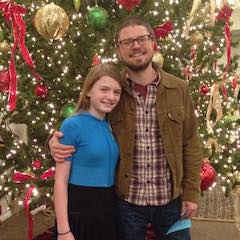
\includegraphics[scale=0.4166666666]{jul_and_me_orig}
		\hspace{0.1cm}
		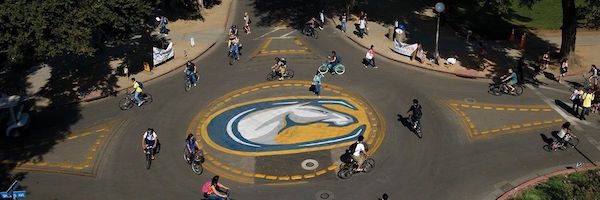
\includegraphics[scale=0.5]{UCD_orig}
		\vspace{0.3cm} \hspace{0.02cm}
		\\
	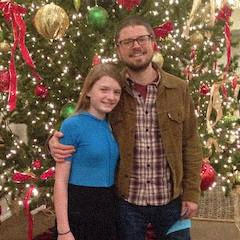
\includegraphics[scale=0.4166666666]{jul_and_me_L_15_ada40}	
		\hspace{0.1cm}
		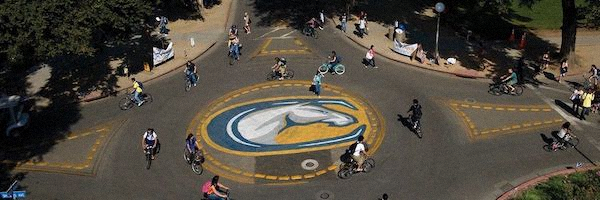
\includegraphics[scale=0.5]{UCD_L_15_ada40} 
		\vspace{0.0cm}
	\caption{
Images used for experiments in Table \ref{Tab:Numerics-ada_vs_orig_large_images}.
Top left: original image of my daughter and me, image size $240 \times 240 = 57,600$ pixels.
Bottom left: result image after solving EMEP.
Top right: original image of UC Davis roundabout, image size $200 \times 600 = 120,000$ pixels.
Bottom right: result image after solving EMEP.
All experiments have noise ratio $\epsilon_\text{rel} = 0.15$ and oversampling $L = 15$.
	}
\label{Fig:Numerics-large_images}
\end{figure}
% experiments.figure.noisyimage_comparison_adaptive_vs_orig


Table \ref{Tab:Numerics-ada_vs_orig_large_images} demonstrates that the benefits of Algorithm \ref{Alg:adaptive_IRAM} also apply to large-scale phase retrieval problems.
Additionally, a larger Arnoldi decomposition size $m$ further reduces the number of matrix-vector products.
Thus, when solving large-scale problems it may be advisable to consider increasing this parameter beyond the default setting of $m=40$ in Algorithm \ref{Alg:adaptive_IRAM} if memory constraints permit this increase.



Next, we demonstrate that Algorithm \ref{Alg:adaptive_IRAM} is nearly optimal in the sense of choosing the number of requested eigenvalues $r_k$ which minimizes the number of matrix-vector products for each \emep \ iterate $k$.
Table \ref{Tab:Numerics-num_matvecs_opt_vs_ada} indicates the number of matrix-vector products for solving the EMEP for six PLGD models with Gaussian noise (\ref{Eqn:PhaseLift-GD_Gaussian_noise}) with Algorithm \ref{Alg:adaptive_IRAM}, with the original IRAM parameters, and with the minimum possible number of matrix-vector products if each value $r_k$ was chosen such that $2 \leq r_k\leq 30$ and $r_k$ corresponds to the minimum number of matrix-vector products for the IRAM to evaluate EMEP iterate $k$.


\begin{table}[H]
\centering
\begin{tabular}{ |ccc|c|cc|cc| }
 \hline
			&&&  Original
			&  \multicolumn{2}{c|}{Optimal $2 \leq r \leq 30$}
			&	\multicolumn{2}{c|}{Algorithm \ref{Alg:adaptive_IRAM}}	\\
$L$ & $\epsilon_\text{rel}$ & EMEP its & $r=2, m=20$	& \multicolumn{2}{c|}{$m=40$}  & \multicolumn{2}{c|}{$m=40$}   \\
 \hline
 5 &  0.05 & 300 &  406,308  &  179,807 & 56\% &  198,070 & 51\% \\ 
  5 &  0.15 & 300 & 1,099,045  &  242,003 & 78\% &  258,385 & 76\% \\ 
  5 &  0.30 &  92 &  444,697  &   58,780 & 87\% &   69,510 & 84\% \\ 
 10 &  0.05 & 153 &   80,453  &   61,948 & 23\% &   68,709 & 15\% \\ 
 10 &  0.15 & 108 &   88,317  &   51,311 & 42\% &   57,231 & 35\% \\ 
 10 &  0.30 &  54 &   72,486  &   23,217 & 68\% &   25,809 & 64\% \\ 
 \hline
\end{tabular}

\caption{
Performance results for PLGD models with Gaussian noise (\ref{Eqn:PhaseLift-GD_Gaussian_noise}) with original signal from Figure \ref{Fig:parrot_signal_iterates} resized to $64 \times 64$ pixels.
Results indicate total number of matrix-vector products and percent decrease from the original IRAM parameters.
Parameter $r$ is the number of requested eigenvalues in the IRAM (Algorithm \ref{Alg:IRAM}) and $m$ is the Arnoldi decomposition size (\ref{Eqn:Arnoldi_decomp}).
} \label{Tab:Numerics-num_matvecs_opt_vs_ada}
\end{table}
% experiments.figure.noisyimage_adaptive_eig_full_exp

Table \ref{Tab:Numerics-num_matvecs_opt_vs_ada} demonstrates that Algorithm \ref{Alg:adaptive_IRAM} decreases the number of matrix-vector products of each PLGD model with Gaussian noise (\ref{Eqn:PhaseLift-GD_Gaussian_noise}) from the original IRAM parameters by a percentage comparable to that of the optimal choice for parameter $r$.
Notably, Algorithm \ref{Alg:adaptive_IRAM} is particularly effective at decreasing the number of matrix-vector products when there is a large relative difference between the number of matrix-vector products for the original IRAM parameters and the optimal parameters.
To further explore this performance behavior, Figure \ref{Fig:Numerics-num_eigs_ada_vs_opt} depicts the two PLGD models from Table \ref{Tab:Numerics-num_matvecs_opt_vs_ada} with the largest and smallest relative difference in matrix-vector products (those with $L=5$, $\epsilon_\text{rel} = 0.15$, and $L=10$, $\epsilon_\text{rel} = 0.05$, respectively).



\begin{figure}[H]
\centering
\hbox{\hspace{-1.8cm} 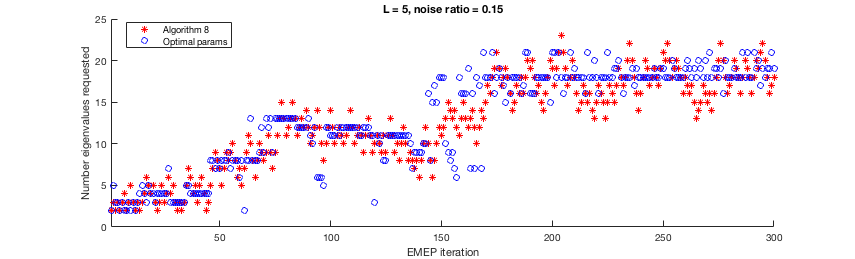
\includegraphics[scale=0.6]{Numerics-num_eigs_ada_vs_opt_1} }\vspace{0.6cm}
\hbox{\hspace{-1.8cm} 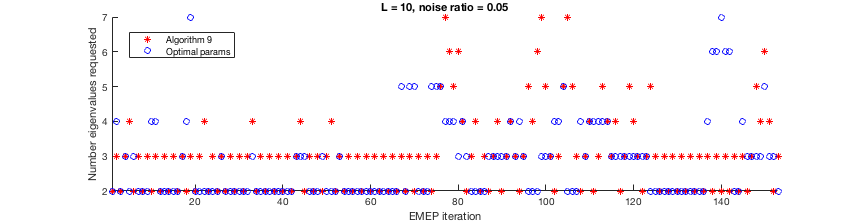
\includegraphics[scale=0.6]{Numerics-num_eigs_ada_vs_opt_2} }
\vspace{0.2cm}
	\caption{
	Number of requested eigenvalues $r$ in the IRAM (Algorithm \ref{Alg:IRAM}) for two PLGD models from Table \ref{Tab:Numerics-num_matvecs_opt_vs_ada}.
	}
\label{Fig:Numerics-num_eigs_ada_vs_opt}
\end{figure}
% experiments.figure.noisyimage_adaptive_eig_full_exp


In both PLGD models depicted in Figure \ref{Fig:Numerics-num_eigs_ada_vs_opt}, the number of requested eigenvalues $r$ chosen by Algorithm \ref{Alg:adaptive_IRAM} is usually within 1-3 units from the optimal parameter value.
The bottom plot in Figure \ref{Fig:Numerics-num_eigs_ada_vs_opt} suggests that Algorithm \ref{Alg:adaptive_IRAM} required relatively more matrix-vector products than the optimal value of $r$ because Algorithm \ref{Alg:adaptive_IRAM} always changes the value of $r$ by one or two units, thus shifting away from the optimal value $r=2$ for many EMEP iterates.
As we saw in Figure \ref{Fig:Numerics-surf_mvs_eig_diffs_2}, the optimal parameter $r$ may shift rapidly for some PLGD models, and thus Algorithm \ref{Alg:adaptive_IRAM} always changes $r$ by one or two units to continue gathering performance information about the EMEP.



%\subsection{Performance results for varying Arnoldi decomposition size}				



Finally, we use performance results to justify selecting $m=40$ as the default Arnoldi decomposition (\ref{Eqn:Arnoldi_decomp}) size for Algorithm \ref{Alg:adaptive_IRAM}.
Table \ref{Tab:Numerics-num_matvecs_orig_vs_ada} depicts the total number of matrix-vector products required to solve the \emep \ for each PLGD model from Table \ref{Tab:Numerics-num_matvecs_opt_vs_ada} with Algorithm \ref{Alg:adaptive_IRAM} with various parameter values $m$.

\begin{table}[H]
\centering
\begin{tabular}{ |ccc|c|ccccc| }
 \hline
			  \multicolumn{3}{|c|}{n = 4,096} &  Original
			&  \multicolumn{5}{c|}{Algorithm \ref{Alg:adaptive_IRAM}}	\\
$L$ & $\epsilon_\text{rel}$ & EMEP its & $r=2, m=20$	& $m=20$  & $m=40$  & $m=60$  & $m=80$  & $m=100$   \\
 \hline
  5 &  0.05 & 300 &  406,308  &  358,195  &  198,070  &  189,401  &  192,042  &  201,270  \\ 
  5 &  0.15 & 300 & 1,099,045  &  806,412  &  258,385  &  224,048  &  214,118  &  215,392  \\ 
  5 &  0.30 &  92 &  444,697  &  175,669  &   69,510  &   56,193  &   55,146  &   54,987  \\ 
 10 &  0.05 & 153 &   80,453  &   77,768  &   68,709  &   64,300  &   68,602  &   73,754  \\ 
 10 &  0.15 & 108 &   88,317  &   65,833  &   57,231  &   53,261  &   54,388  &   55,308  \\ 
 10 &  0.30 &  54 &   72,486  &   28,799  &   25,809  &   24,699  &   25,113  &   25,491  \\ 
 \hline
\end{tabular}

\caption{
Total number of matrix-vector products for various PLGD models with Gaussian noise	(\ref{Eqn:PhaseLift-GD_Gaussian_noise}) with original signal from Figure \ref{Fig:parrot_signal_iterates} resized to $64 \times 64$ pixels.
Parameter $r$ is the number of requested eigenvalues in the IRAM (Algorithm \ref{Alg:IRAM}) and $m$ is the Arnoldi decomposition (\ref{Eqn:Arnoldi_decomp}) size. 
} \label{Tab:Numerics-num_matvecs_orig_vs_ada}
\end{table}
% experiments.figure.noisyimage_adaptive_eig_full_exp



Table \ref{Tab:Numerics-num_matvecs_orig_vs_ada} demonstrates that Algorithm \ref{Alg:adaptive_IRAM} reduces the number of matrix-vector products from those of the original IRAM parameters for all experiments considered.
Yet this cost reduction varies significantly depending on the choice of Arnoldi decomposition (\ref{Eqn:Arnoldi_decomp}) size $m$.
We seek a default setting for the parameter $m$ which is sufficiently large to yield the benefits of Algorithm \ref{Alg:adaptive_IRAM}, yet sufficiently small as not to impact memory constraints.
To select an appropriate default value for $m$, we examine the two experiments from Table \ref{Tab:Numerics-num_matvecs_orig_vs_ada} with $\epsilon_\text{rel} = 0.15, 0.30$ and $L=5$ which have the greatest original number of matrix-vector products, along with the greatest total decrease in cost when using Algorithm \ref{Alg:adaptive_IRAM} with a sufficiently large parameter $m$.
Figure \ref{Fig:Numerics-num_matvecs_ada_for_m_vals} singles out these two experiments, depicting the number of matrix-vector products for each \emep \ iteration.

\begin{figure}[H]
\centering
\hbox{\hspace{-1.6cm} 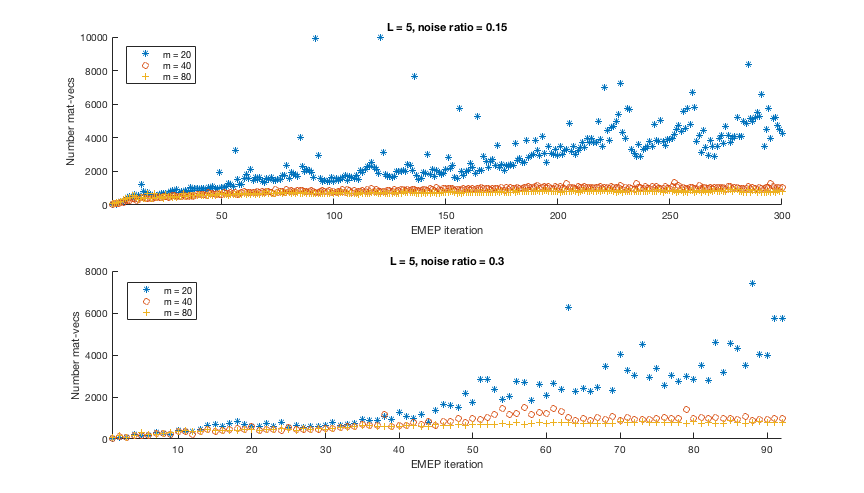
\includegraphics[scale=0.6]{Numerics-num_matvecs_ada_for_m_vals} }\vspace{0.0cm}
	\caption{Number of matrix-vector products for each \emep \ iteration from two experiments in Figure \ref{Fig:Numerics-num_matvecs_ada_for_m_vals} with various Arnoldi decomposition size $m=20, 40, 80$.}
\label{Fig:Numerics-num_matvecs_ada_for_m_vals}
\end{figure}
% experiments.figure.noisyimage_adaptive_eig_full_exp




Figure \ref{Fig:Numerics-num_matvecs_ada_for_m_vals} demonstrates that the Arnoldi decomposition size of $m=20$ is not sufficiently large to allow Algorithm \ref{Alg:adaptive_IRAM} to decrease the number of matrix-vector products.  
The dramatic matrix-vector product spikes for $m=20$ in Figure \ref{Fig:Numerics-num_matvecs_ada_for_m_vals} resemble those first seen in Figure \ref{Fig:EMEP_costs_num_mat_vecs} when solving the \emep \ with the original IRAM parameters $m=20, r=2$.
Yet when the Arnoldi decomposition size is increased to $m=40$, these cost spikes effectively disappear.
The change in number of matrix-vector products between $m=40$ and $m=80$ is minimal for each EMEP iterate.  
Thus the default parameter of $m=40$ for Algorithm \ref{Alg:adaptive_IRAM} strikes the proper balance between efficiency and memory constraints.





\section{Contributions and future work} 			\label{Subsec:Conclusion-contrib_and_future}


In this dissertation we examined noisy phase retrieval, focusing on the PLGD model (\ref{Eqn:PhaseLift-P-GD}) which we chose to optimize with Algorithm \ref{Alg:PGD} from Chapter \ref{Sec:PLGD_algo}.
Our work offers two primary contributions.


First, we established new termination conditions for Algorithm \ref{Alg:PGD}.
Chapter \ref{Sec:PLGD_term_crit} showed that PLGD models with Gaussian noise (\ref{Eqn:PhaseLift-GD_Gaussian_noise}) cause Algorithm \ref{Alg:PGD} to stagnate prior to satisfying the original termination conditions (\ref{Eqn:saga_conv_crit_primal}) and (\ref{Eqn:saga_conv_crit_gap}).  
We saw that this stagnation was likely the result of the optimal PLGD matrix $\caA^*y_\star$ having an algebraically largest eigenvalue with multiplicity greater than one.
Thus the objective function $\lambda_1(\caA^*y)$ will be nondifferentiable in the neighborhood of $y_\star$ and we may expect first-order methods like Algorithm \ref{Alg:PGD} to stagnate in this neighborhood.
As a result, we established new termination conditions (\ref{Eqn:term_crit_new-primal_difference}) and (\ref{Eqn:term_crit_new-dual_difference}) based on empirical evidence of algorithmic stagnation.


Second, we developed a new strategy for handling the \emep \ in Algorithm \ref{Alg:PGD}.
In Chapter \ref{Sec:evol_mats} we defined the EMEP in Algorithm \ref{Alg:PGD} and examined the evolving spectrum of the EMEP.
We observed that the algebraically largest eigenvalues of the EMEP tend to cluster for later iterates, making these eigenvalue problems more difficult for methods like the IRAM (Algorithm \ref{Alg:IRAM}).
We also showed that the EMEP is the computational bottleneck of Algorithm \ref{Alg:PGD}, requiring about $95$\% of the matrix-vector products in Algorithm \ref{Alg:PGD}.
Section \ref{Subsec:evol_mats-IRAM} then reviewed the IRAM and its component algorithms, providing insight for how we may better select the IRAM parameters.
Next, Chapter \ref{Sec:Numerics} developed Algorithm \ref{Alg:adaptive_IRAM}, a new strategy for solving the EMEP by selecting the number of requested eigenvalues in the IRAM based on empirical observations of IRAM behavior.
Section \ref{Subsec:Numerics-correl_btwn_EMEP_and_IRAM} showed that changes in the number of requested eigenvalues, as chosen by Algorithm \ref{Alg:adaptive_IRAM}, correspond to clustering of the algebraically largest eigenvalues in the EMEP.
Performance results in Section \ref{Subsec:Conclusion-performance_results} demonstrated that Algorithm \ref{Alg:adaptive_IRAM} is more efficient than the original parameter selection used for the EMEP, reducing the number of matrix-vector products by $50$-$90\%$.


In addition to these contributions, Chapter \ref{Sec:PLGD} presented a self-contained, comprehensive treatment of gauge duality theory for establishing and analyzing the PLP-PLGD pair and Section \ref{Subsec:phase_retrieval-why_optimize_PLGD_model} justified the choice of the PLGD model (\ref{Eqn:PhaseLift-P-GD}) for noisy phase retrieval.


Several theoretical and computational questions still remain for future work.  
In terms of theory, it would be beneficial to determine the expected rank of a given optimal PLGD matrix $\caA^*y_\star$. 
As mentioned above, PLGD models with Gaussian noise typically have matrices $\caA^*y_\star$ with rank $\rho$ greater than one (see Table \ref{Tab:average_rank_soln_matrix_with_gaussian_dual_variable}).
Thus, as Algorithm \ref{Alg:PGD} progresses we may expect the $\rho$ algebraically largest eigenvalues of $\caA^*y$ to cluster.
Algorithm \ref{Alg:adaptive_IRAM} changes the number of requested eigenvalues $r$ in the IRAM (Algorithm \ref{Alg:IRAM}) as the spectrum of $\caA^*y$ evolves.
As we saw in Section \ref{Subsec:Numerics-correl_btwn_EMEP_and_IRAM}, changes in the choice of $r$ appear to correlate with clustering of the algebraically largest eigenvalues of $\caA^*y$.
In this sense, the value $r$ selected by Algorithm \ref{Alg:adaptive_IRAM} may be a proxy for determining the rank $\rho$ of $\caA^*y_\star$.
Knowledge of the expected value for $\rho$ may provide both theoretical justification for Algorithm \ref{Alg:adaptive_IRAM} and a means to modify and enhance Algorithm \ref{Alg:adaptive_IRAM}.


Many computational questions also remain for future work.
In terms of solving the \emep, we did not examine parallel methods for solving this sequence of problems.\footnote{
Note that we did consider the \textit{inverse free preconditioned Krylov subspace method} (EIGIFP) \cite{golub2002inverse}, which was comparable to or slightly slower than IRAM.  EIGIFP is implemented in MATLAB and this code had some numerical issues for larger PLGD models.
}
We also did not discuss optimizing the method for handling the primal recovery problem (\ref{Eqn:GD-PFD}) in Algorithm \ref{Alg:PGD}.
Recall that the primal recovery problem requires $2$-$5\%$ of the total DFTs in a given PLGD model (see Table \ref{Tab:EMEP_costs}).
The current method used is \textit{minFunc} \cite{schmidt2005minFunc}, which is a quasi-Newton method based only on gradient information.
However, a recent paper \cite{sun2016geometric} indicates that the objective function in (\ref{Eqn:GD-PFD}) has no spurious local minima and negative directional curvature at all saddle points.
Thus the Hessian of this function may also be used to solve (\ref{Eqn:GD-PFD}).
Finally, we did not discuss alternative methods to Algorithm \ref{Alg:PGD} for optimizing the PLGD model itself.\footnote{
Note that we did consider \textit{minConf} \cite{schmidt2008minConf}, a descent method for problems like the PLGD model with an expensive objective function and cheap projection operator.  This method appeared comparable to Algorithm \ref{Alg:PGD} and in some cases faster.
}






